\documentclass[12pt,a4paper]{article}

\usepackage{amssymb}
\usepackage{amsmath}
\usepackage{graphicx}
\usepackage{booktabs}
\usepackage{multirow}
\usepackage{hyperref}
\usepackage{float}
\usepackage{xcolor}
\usepackage{geometry}
\usepackage{natbib}
\usepackage{authblk}
\usepackage{abstract}
\usepackage{enumitem}

\geometry{left=2.5cm, right=2.5cm, top=2.5cm, bottom=2.5cm}

\renewcommand{\abstractnamefont}{\normalfont\bfseries}
\renewcommand{\abstracttextfont}{\normalfont\small}

\title{\textbf{A Machine Learning and Deep Perceptron Approach for Mortality Risk Prediction and Clinical Risk Factor Analysis of Heart Failure Patients}}

\author[1]{Author A\thanks{Corresponding author. E-mail: authora@university.edu}}
\author[1]{Author B}
\author[2]{Author C}
\affil[1]{Department of Computer Science, University A, City, Country}
\affil[2]{Department of Cardiology, University B, City, Country}

\date{}

\begin{document}

\maketitle

\begin{abstract}
\noindent
In this study, we propose a multi-model machine learning (ML) pipeline for mortality risk prediction and clinical risk factor analysis of Heart Failure (HF) patients using a clinical records dataset of 299 patients. Four models are applied and compared: Random Forest (RF), Logistic Regression (LR), XGBoost, and a deep Multi-Layer Perceptron (MLP) neural network built with PyTorch. Model performances are evaluated on a held-out test set using accuracy, precision, recall, $F_1$ score, and the area under the receiver operating characteristic curve (AUC). Results show that RF achieves the best overall performance with an AUC of 0.9024 and an accuracy of 85.00\%. Risk factor analysis is conducted through three independent approaches: Pearson correlation analysis, Welch's $t$-test, and Gini-based feature importance from RF. The three methods consistently identify follow-up time, serum creatinine (SC), and ejection fraction (EF) as the top three risk factors for HF mortality. A clinical inference module further demonstrates the pipeline's capability for individualized probability prediction on new patients. Our results suggest that ensemble tree-based methods outperform both linear models and deep learning on small-sample structured clinical data, and that the identified risk factors are consistent with established clinical knowledge of cardiorenal syndrome and left ventricular systolic dysfunction.

\vspace{0.5em}
\noindent\textbf{Keywords:} Machine learning; Heart failure; Risk factor analysis; Feature importance; Deep learning; Survival prediction
\end{abstract}

%% ============================================================
\section{Introduction}
\label{sec:intro}

Cardiovascular diseases (CVDs), including coronary heart disease, strokes, and heart failure (HF), constitute a leading global burden of disease \citep{chicco2020ml}. HF occurs when the heart is unable to pump sufficient blood to meet the body's metabolic demands, often precipitated by hypertension, diabetes, coronary artery disease, or other cardiac disorders \citep{ali2023ml}. According to the World Health Organization, CVDs account for approximately 31\% of all deaths worldwide.

Accurate prognostic assessment of HF patients is essential for timely clinical intervention---such as intensified pharmacotherapy or surgical planning---and for the efficient allocation of medical resources. Previous studies have explored HF survival prediction using various approaches. Pocock et al.\ \citep{pocock2006} developed a prognostic model using multivariate Cox regression and identified 21 predictor variables, though the model lacked the computational efficiency of modern ML algorithms. Chicco and Jurman \citep{chicco2020ml} demonstrated that survival prediction is feasible using serum creatinine (SC) and ejection fraction (EF) alone, yet relying on only two features may underrepresent the multifactorial nature of HF mortality. Ahmad et al.\ \citep{ahmad2017} proposed a Cox regression-based survival model but did not validate computational cost or classification performance. Ali et al.\ \citep{ali2023ml} applied five supervised ML methods and achieved 97.78\% accuracy with Random Forest, identifying SC, age, EF, platelets, CPK, and serum sodium (SS) as the top six risk factors.

Despite these efforts, limited work has systematically compared traditional ML, gradient boosting, and deep learning approaches on the same HF dataset while simultaneously conducting multi-method risk factor validation. This study addresses this gap by constructing an end-to-end data analysis and modeling pipeline based on clinical records of 299 HF patients. The main contributions are as follows:

\begin{enumerate}[label=(\alph*)]
    \item Building a multi-model comparison framework including Random Forest, Logistic Regression, XGBoost, and a deep MLP neural network, with hyperparameter tuning and rigorous evaluation on a held-out test set.
    \item Cross-validating risk factor identification through three independent methods: Pearson correlation, Welch's $t$-test, and Gini-based feature importance.
    \item Demonstrating clinical inference capability through individualized mortality probability prediction for new patients.
    \item Providing methodological insights on when deep learning is outperformed by ensemble methods on small-sample tabular clinical data.
\end{enumerate}

The overall conceptual framework of our AI-assisted heart failure risk prediction system is illustrated in Fig.~\ref{fig:concept_framework}, which integrates clinical data sources, machine learning modeling, risk interpretation, and clinical decision support into a unified pipeline.

\begin{figure}[H]
\centering
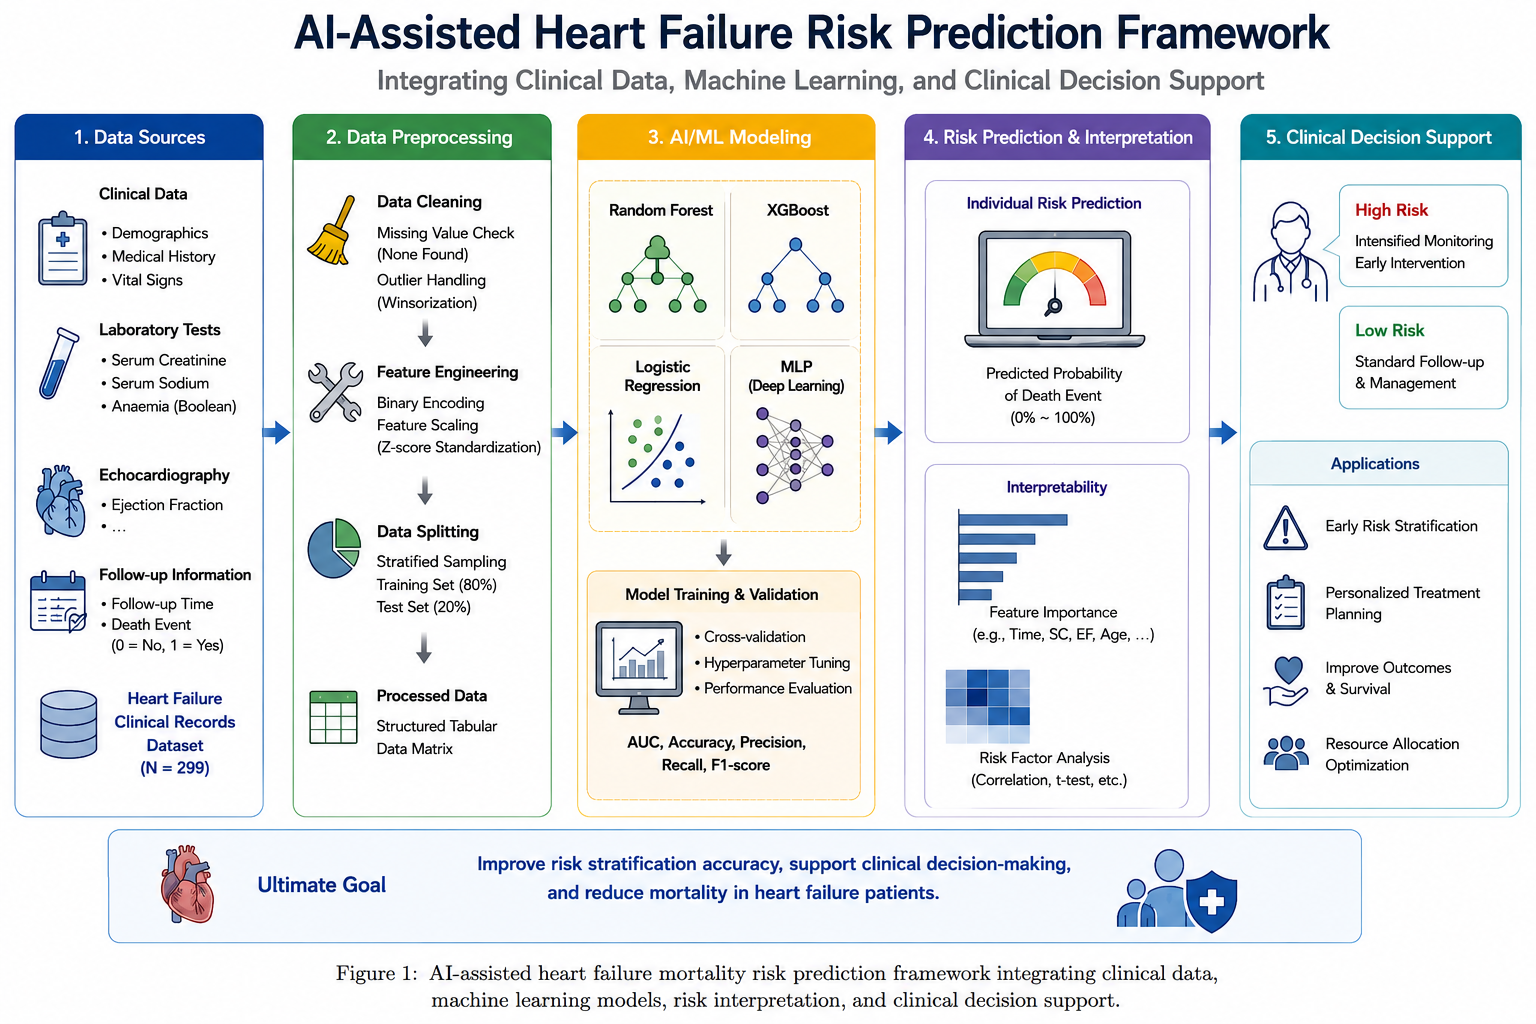
\includegraphics[width=\textwidth]{AI-assisted_heart_faliure_risk_prediction_diagram.png}
\caption{AI-assisted heart failure mortality risk prediction concept framework integrating clinical data, machine learning models, risk interpretation, and clinical decision support.}
\label{fig:concept_framework}
\end{figure}

%% ============================================================
\section{Materials and Methods}
\label{sec:methods}

The overall research methodology is depicted in Fig.~\ref{fig:pipeline_description}. The study was implemented using Python~3 with scikit-learn, XGBoost, and PyTorch libraries.

\begin{figure}[H]
\centering
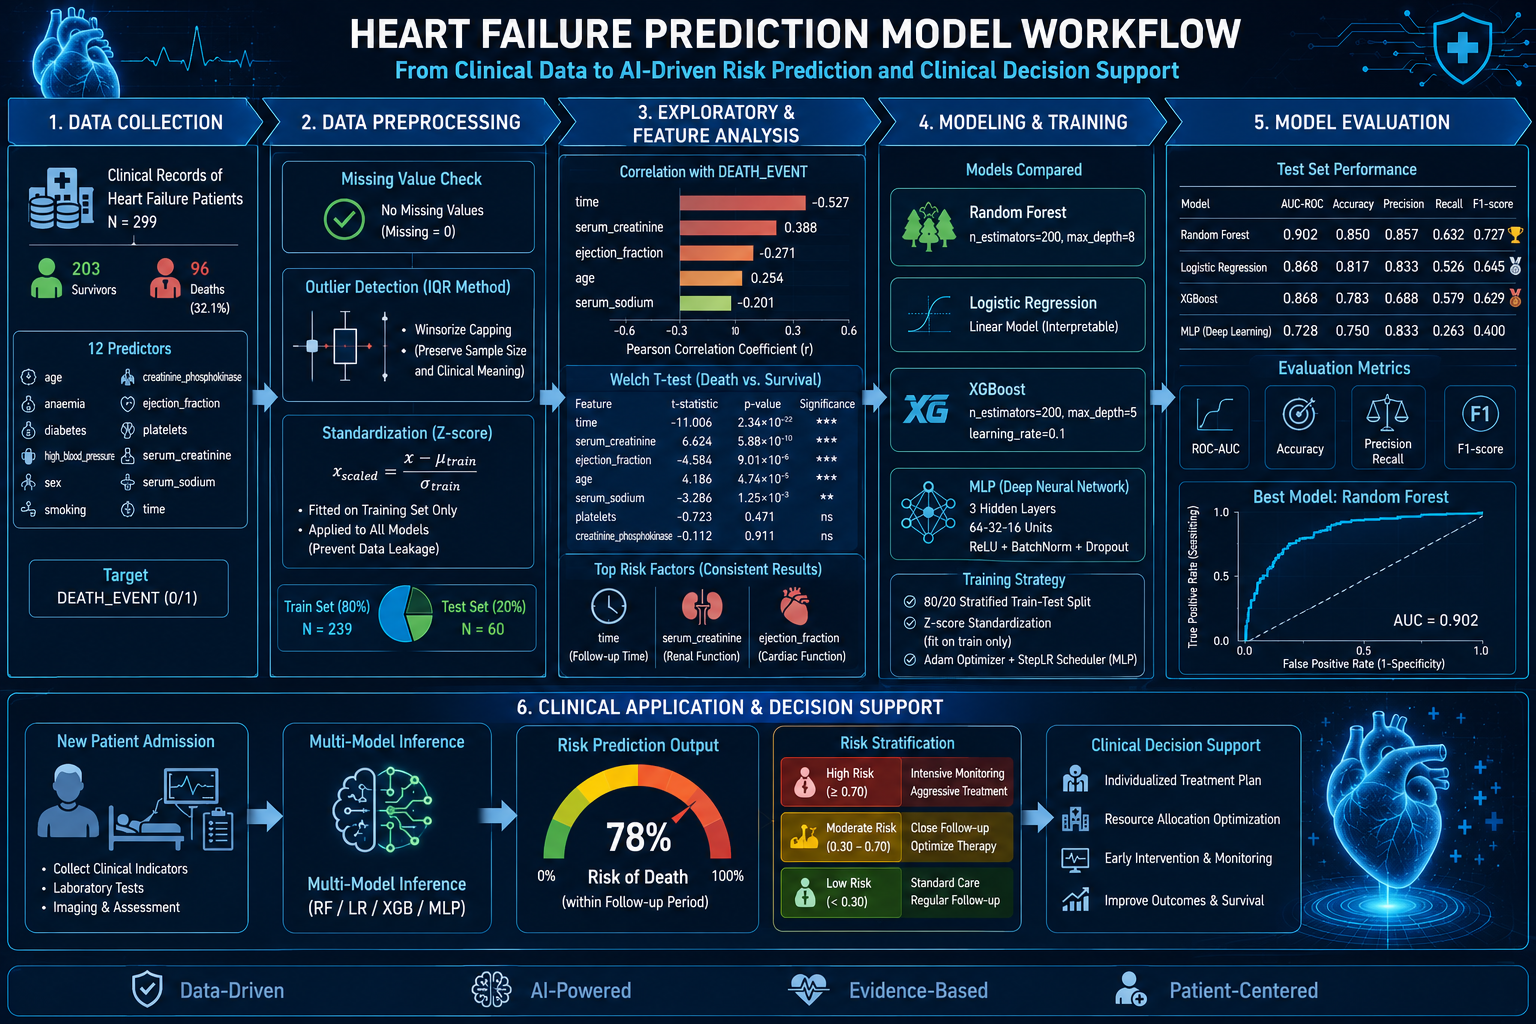
\includegraphics[width=\textwidth]{Working_flow_chart_of_heart_faliure_prediction_model.png}
\caption{Pipeline of the proposed ML models and data analysis framework. The workflow encompasses six stages: data collection, data preprocessing, exploratory and feature analysis, modeling and training, model evaluation, and clinical application and decision support.}
\label{fig:pipeline_description}
\end{figure}

\subsection{Dataset Description}

The dataset used in this study is a publicly available HF clinical records dataset originally collected by Ahmad et al.\ \citep{ahmad2017}. It contains 299 patient records with 12 predictor variables and one binary target variable (\texttt{DEATH\_EVENT}). Among these, 203 patients survived and 96 died during the follow-up period (mortality rate $\approx$ 32.1\%). The detailed data description is provided in Table~\ref{tab:data_description}.

\begin{table}[H]
\centering
\caption{Data description of the HF clinical records dataset.}
\label{tab:data_description}
\small
\begin{tabular}{lll}
\toprule
\textbf{Feature Name} & \textbf{Type} & \textbf{Description} \\
\midrule
Age              & Float   & Age of the patient (years) \\
Anaemia          & Boolean & Decrease of red blood cells or hemoglobin \\
CPK              & Integer & Level of creatinine phosphokinase in blood (mcg/L) \\
Diabetes         & Boolean & Whether the patient has diabetes \\
EF               & Integer & Percentage of blood leaving the heart per contraction (\%) \\
HBP              & Boolean & Whether the patient has high blood pressure \\
Platelets        & Float   & Platelet count in blood (kiloplatelets/mL) \\
SC               & Float   & Level of serum creatinine in blood (mg/dL) \\
SS               & Integer & Level of serum sodium in blood (mEq/L) \\
Sex              & Boolean & Male (1) or Female (0) \\
Smoking          & Boolean & Whether the patient smokes \\
Time             & Integer & Follow-up period (days) \\
DEATH\_EVENT     & Boolean & Target: died during follow-up (1) or survived (0) \\
\bottomrule
\end{tabular}
\end{table}

\subsubsection{Class Distribution Analysis}

The dataset contains 299 heart failure patients, including 203 survivors and 96 deceased patients. The corresponding mortality rate is 32.1\%, while the survival rate is 67.9\%. Although the imbalance is not extreme, the dataset exhibits a moderate class imbalance that may influence model training and evaluation.

To ensure that both classes are proportionally represented in the training and testing datasets, stratified sampling was adopted during data partitioning. This approach preserves the original class distribution and reduces the risk of biased performance estimation caused by uneven class representation. Table~\ref{tab:class_distribution} summarizes the class distribution of the dataset.

\begin{table}[H]
\centering
\caption{Class distribution of the HF dataset.}
\label{tab:class_distribution}
\begin{tabular}{lrc}
\toprule
\textbf{Class} & \textbf{Count} & \textbf{Percentage} \\
\midrule
Survived & 203 & 67.9\% \\
Deceased & 96  & 32.1\% \\
\midrule
Total    & 299 & 100.0\% \\
\bottomrule
\end{tabular}
\end{table}

\subsection{Data Preprocessing}

\subsubsection{Missing Value Detection}

An automated screening confirmed that the dataset contains \textbf{no missing values} across all 13 columns, ensuring sample consistency for subsequent analysis without the need for imputation methods that could introduce stochastic bias.

\subsubsection{Outlier Detection and Treatment}

Outlier detection was performed on all seven continuous variables using the \textbf{Interquartile Range (IQR) method}. An observation was defined as an outlier if it fell below $Q_1 - 1.5 \times \mathrm{IQR}$ or above $Q_3 + 1.5 \times \mathrm{IQR}$. The detection results are summarized in Table~\ref{tab:outlier_detection}.

\begin{table}[H]
\centering
\caption{Outlier detection results for continuous variables (IQR method).}
\label{tab:outlier_detection}
\small
\begin{tabular}{lrrrrrc}
\toprule
\textbf{Feature} & $\mathbf{Q_1}$ & $\mathbf{Q_3}$ & \textbf{IQR} & \textbf{Lower} & \textbf{Upper} & \textbf{Outliers} \\
\midrule
Age    & 51.0  & 70.0  & 19.0  & 22.5   & 98.5   & 0  \\
CPK    & 116.5 & 582.0 & 465.5 & $-$581.8 & 1280.3 & 29 \\
EF     & 30.0  & 45.0  & 15.0  & 7.5    & 67.5   & 2  \\
Platelets & 212\,500 & 303\,500 & 91\,000 & 76\,000 & 440\,000 & 21 \\
SC     & 0.9   & 1.4   & 0.5   & 0.15   & 2.15   & 29 \\
SS     & 134.0 & 140.0 & 6.0   & 125.0  & 149.0  & 4  \\
Time   & 73.0  & 203.0 & 130.0 & $-$122.0 & 398.0  & 0  \\
\bottomrule
\end{tabular}
\end{table}

Rather than deleting outliers, this study applied \textbf{Winsorization}---capping extreme values at the IQR boundaries. This strategy was chosen for two reasons: (1)~the dataset contains only 299 records with an imbalanced class distribution (96 deaths), so deletion would further reduce minority class representation; (2)~clinically, extreme values of CPK and SC often reflect genuine pathological states (e.g., acute myocardial injury or acute renal deterioration) rather than measurement errors, and Winsorization preserves this clinical signal while mitigating undue leverage on model estimation.

\subsubsection{Train-Test Split}

To evaluate model generalization performance, the dataset was divided into training and testing subsets using stratified random sampling. Eighty percent of the samples were allocated to the training set ($n = 239$), while the remaining 20\% were reserved for independent testing ($n = 60$).

Stratified sampling was employed to maintain the original class distribution of the mortality outcome in both subsets. This strategy is particularly important for moderately imbalanced clinical datasets, as it prevents the underrepresentation of minority-class samples during model training and evaluation. Table~\ref{tab:train_test_split} presents the sample allocation used in this study.

\begin{table}[H]
\centering
\caption{Train-test split allocation.}
\label{tab:train_test_split}
\begin{tabular}{lrc}
\toprule
\textbf{Dataset Subset} & \textbf{Samples} & \textbf{Percentage} \\
\midrule
Training Set & 239 & 80\% \\
Test Set     & 60  & 20\% \\
\midrule
Total        & 299 & 100\% \\
\bottomrule
\end{tabular}
\end{table}

\subsubsection{Feature Standardization}

Following the train-test split described above, all features were standardized using $Z$-score normalization:

\begin{equation}
\label{eq:zscore}
x_{\mathrm{scaled}} = \frac{x - \mu_{\mathrm{train}}}{\sigma_{\mathrm{train}}}
\end{equation}

\noindent where $\mu_{\mathrm{train}}$ and $\sigma_{\mathrm{train}}$ are the mean and standard deviation computed \emph{only} on the training set; the same parameters are applied to the test set to prevent data leakage.

Tree-based models (Random Forest, XGBoost) are inherently scale-invariant, as their splitting criteria depend on relative feature ordering. However, gradient-based models (Logistic Regression, MLP) require standardization to ensure stable convergence and uniform $L_2$ regularization across features. For fair comparison, all models received standardized inputs.

\subsection{Risk Factor Detection and Feature Engineering}

\subsubsection{Pearson Correlation Analysis}

A global correlation heatmap (Fig.~\ref{fig:correlation_heatmap}) was computed to examine linear associations. The Pearson correlation coefficients (absolute values) between each feature and the target variable \texttt{DEATH\_EVENT} are ranked in Table~\ref{tab:correlation_ranking}.

\begin{figure}[H]
\centering
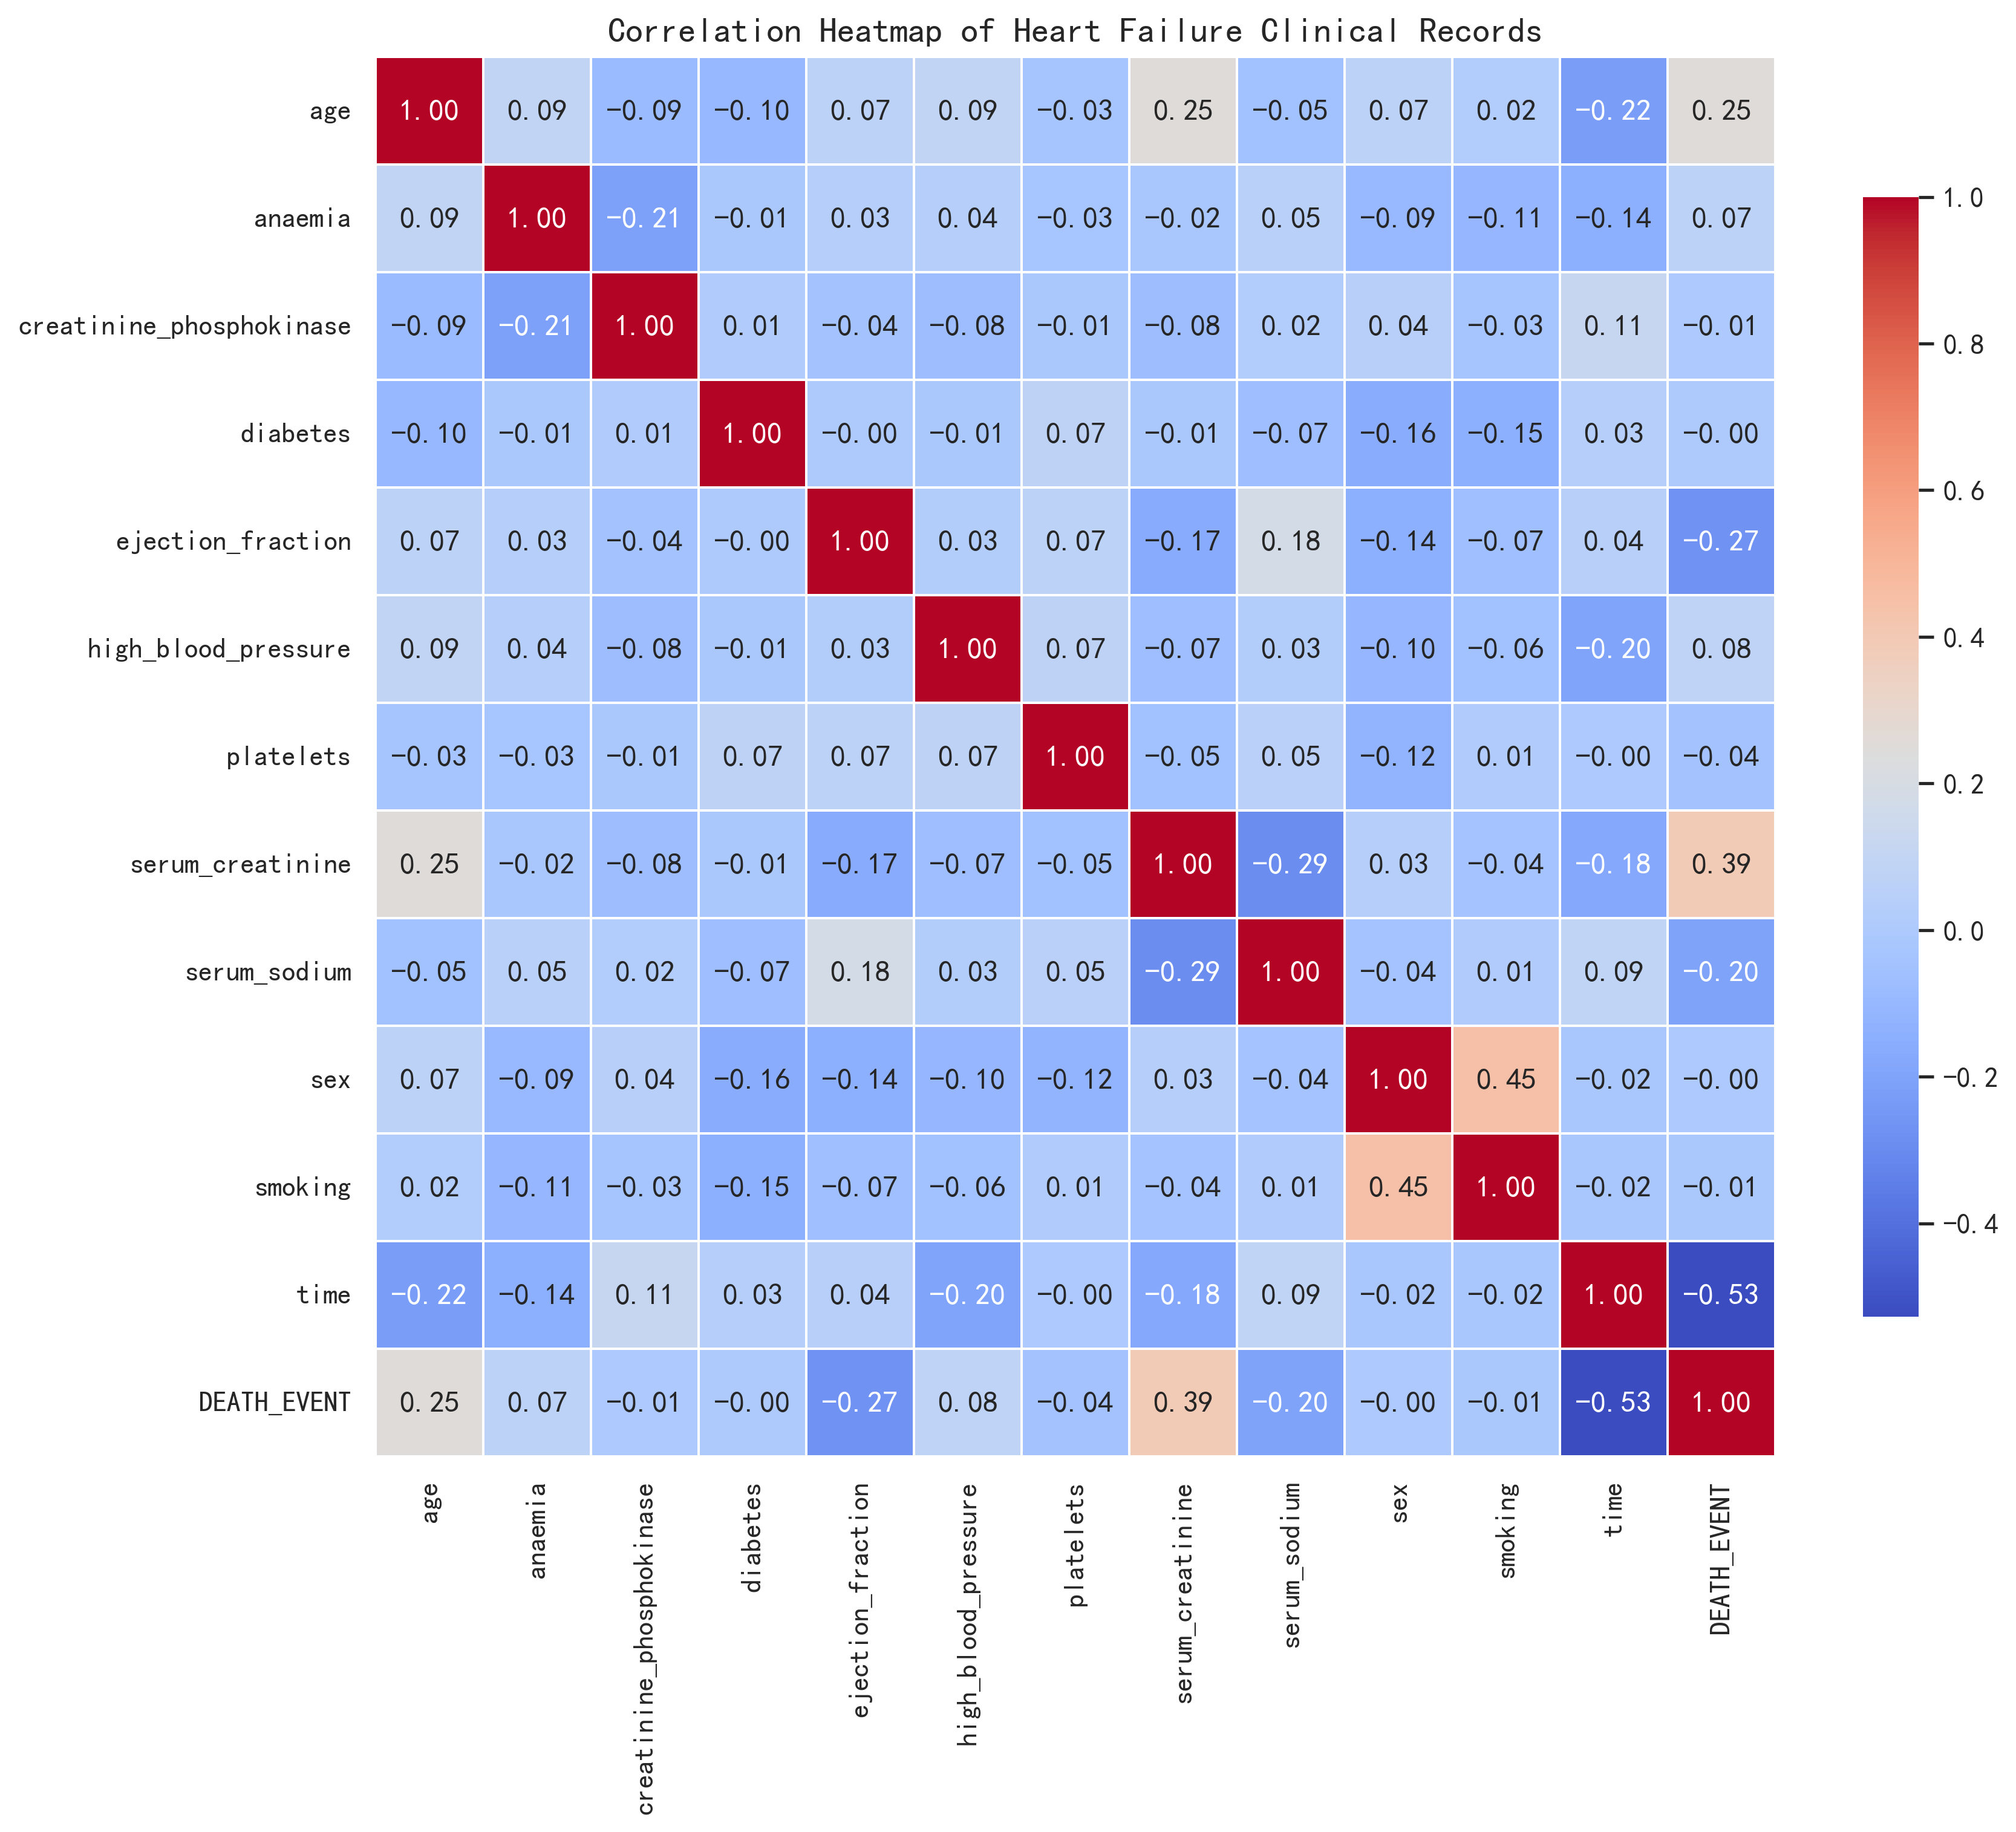
\includegraphics[width=0.85\textwidth]{correlation_heatmap.png}
\caption{Correlation heatmap of Heart Failure clinical records. The color intensity indicates the strength and direction of pairwise Pearson correlation coefficients among all features and the target variable \texttt{DEATH\_EVENT}.}
\label{fig:correlation_heatmap}
\end{figure}

\begin{table}[H]
\centering
\caption{Pearson correlation coefficients between features and \texttt{DEATH\_EVENT} (absolute values, ranked).}
\label{tab:correlation_ranking}
\begin{tabular}{clc}
\toprule
\textbf{Rank} & \textbf{Feature} & $|\mathbf{r}|$ \\
\midrule
1 & Time (follow-up period)       & 0.527 \\
2 & Serum creatinine (SC)         & 0.388 \\
3 & Ejection fraction (EF)        & 0.271 \\
4 & Age                           & 0.254 \\
5 & Serum sodium (SS)             & 0.201 \\
\bottomrule
\end{tabular}
\end{table}

Binary categorical features (e.g., smoking, diabetes, sex) exhibited weak linear correlations with the target ($|r| < 0.10$), suggesting that their contributions may arise through nonlinear interactions or become apparent only after adjusting for confounders.

\subsubsection{Welch's Independent Samples $t$-Test}

To assess whether the differences in continuous variables between the deceased and survived groups are statistically significant, \textbf{Welch's $t$-test} (which does not assume equal variances) was applied. The results are presented in Table~\ref{tab:ttest_results}.

\begin{table}[H]
\centering
\caption{Welch's $t$-test results comparing deceased and survived groups.}
\label{tab:ttest_results}
\small
\begin{tabular}{lrrrl}
\toprule
\textbf{Feature} & \textbf{Dead (Mean)} & \textbf{Survived (Mean)} & $\mathbf{t}$\textbf{-statistic} & \textbf{$p$-value} \\
\midrule
Time   & 70.89    & 158.34   & $-$11.006 & $2.34 \times 10^{-22}$ *** \\
SC     & 1.48     & 1.12     & 6.624     & $5.88 \times 10^{-10}$ *** \\
EF     & 33.44    & 40.20    & $-$4.584  & $9.01 \times 10^{-6}$  *** \\
Age    & 65.22    & 58.76    & 4.186     & $4.74 \times 10^{-5}$  *** \\
SS     & 135.52   & 137.28   & $-$3.286  & $1.25 \times 10^{-3}$  **  \\
Platelets & 253\,944 & 261\,632 & $-$0.723 & 0.471 \hspace{1em} ns \\
CPK    & 420.66   & 425.90   & $-$0.112  & 0.911 \hspace{1em} ns \\
\bottomrule
\multicolumn{5}{l}{\footnotesize *** $p<0.001$, ** $p<0.01$, * $p<0.05$, ns = not significant.}
\end{tabular}
\end{table}

Time, SC, EF, and age all reached $p < 0.001$, and SS reached $p < 0.01$. Notably, platelets and CPK showed non-significant $t$-test results despite moderate Random Forest importance scores, indicating that their predictive contributions arise primarily from nonlinear interaction effects rather than simple mean-level differences.

\subsubsection{Random Forest Feature Importance}

A Random Forest classifier (\texttt{n\_estimators}$\,=200$) was trained, and feature importance was assessed using the Mean Decrease in Impurity (MDI, Gini importance). The ranked results are presented in Table~\ref{tab:feature_importance} and visualized in Fig.~\ref{fig:feature_importance}.

\begin{figure}[H]
\centering
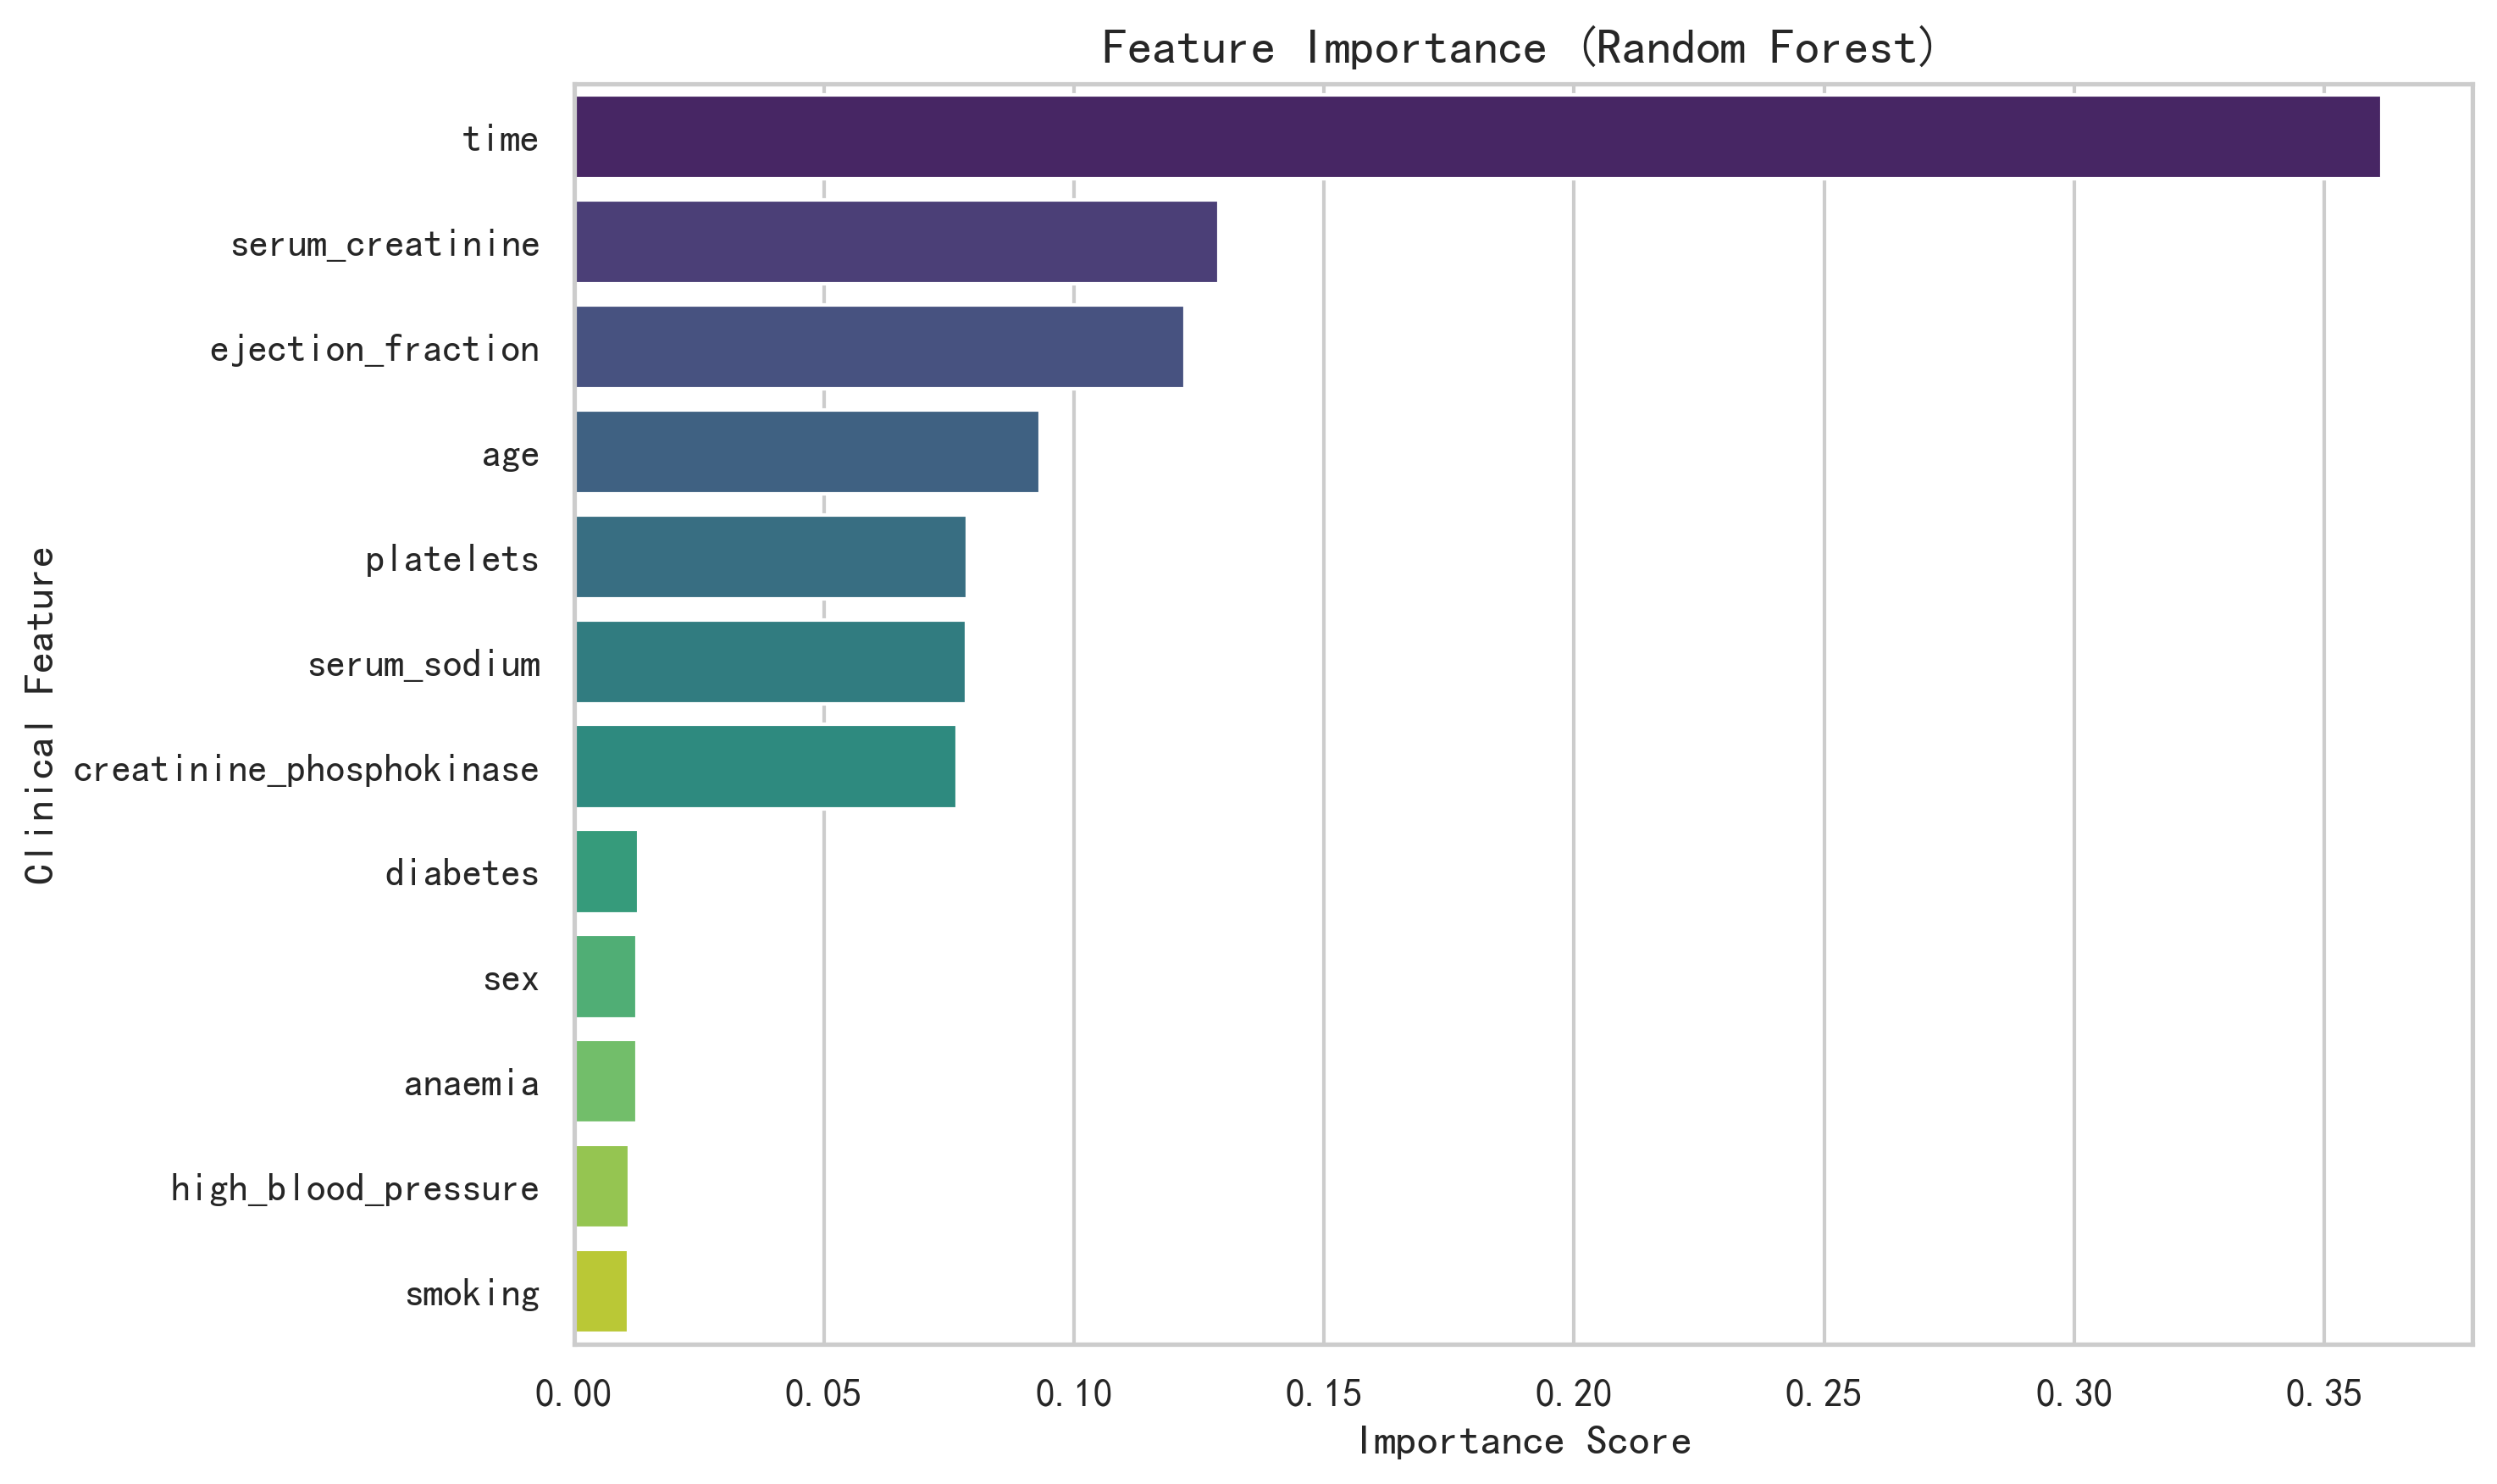
\includegraphics[width=0.9\textwidth]{feature_importance.png}
\caption{Feature importance ranking for HF death event prediction using Random Forest classifier. Follow-up time, serum creatinine, and ejection fraction are the top three contributors.}
\label{fig:feature_importance}
\end{figure}

\begin{table}[H]
\centering
\caption{Random Forest Gini-based feature importance scores (ranked).}
\label{tab:feature_importance}
\begin{tabular}{clc}
\toprule
\textbf{Rank} & \textbf{Feature} & \textbf{Importance} \\
\midrule
1 & Time (follow-up period)         & 0.362 \\
2 & Serum creatinine (SC)           & 0.129 \\
3 & Ejection fraction (EF)          & 0.122 \\
4 & Age                             & 0.093 \\
5 & Platelets                       & 0.079 \\
6 & Serum sodium (SS)               & 0.079 \\
7 & Creatinine phosphokinase (CPK)  & 0.077 \\
\bottomrule
\end{tabular}
\end{table}

The top three risk factors---follow-up time, SC, and EF---are consistent across all three analytical methods (Pearson correlation, Welch's $t$-test, and RF feature importance), providing cross-validated evidence for their clinical relevance.

\subsection{Predictive Modeling}

\subsubsection{Model Selection and Hyperparameters}

Four models were constructed for comparative evaluation. The hyperparameter configurations are summarized in Table~\ref{tab:hyperparams}.

\begin{table}[H]
\centering
\caption{Hyperparameter configurations for all applied models.}
\label{tab:hyperparams}
\begin{tabular}{ll}
\toprule
\textbf{Model} & \textbf{Hyperparameters} \\
\midrule
Random Forest       & \texttt{n\_estimators}$\,=200$, \texttt{max\_depth}$\,=8$ \\
Logistic Regression & \texttt{max\_iter}$\,=1000$, $L_2$ penalty (default) \\
XGBoost             & \texttt{n\_estimators}$\,=200$, \texttt{max\_depth}$\,=5$, \texttt{lr}$\,=0.1$ \\
MLP (PyTorch)       & 3 hidden layers (64--32--16), Adam, \texttt{lr}$\,=0.003$, 150 epochs \\
\bottomrule
\end{tabular}
\end{table}

\paragraph{Multi-Layer Perceptron (MLP) Architecture.}
The MLP was implemented in PyTorch as a three-hidden-layer feedforward neural network:

\begin{equation}
\label{eq:mlp_arch}
\mathrm{Input}(12) \!\to\! \mathrm{FC}(64) \!\to\! \mathrm{BN} \!\to\! \mathrm{ReLU} \!\to\! \mathrm{Drop}(0.3) \!\to\! \mathrm{FC}(32) \!\to\! \mathrm{BN} \!\to\! \mathrm{ReLU} \!\to\! \mathrm{Drop}(0.2) \!\to\! \mathrm{FC}(16) \!\to\! \mathrm{ReLU} \!\to\! \mathrm{FC}(1) \!\to\! \sigma
\end{equation}

\noindent where FC denotes a fully connected layer, BN denotes batch normalization, Drop denotes dropout, and $\sigma$ denotes the sigmoid activation. The network was trained with the Adam optimizer (learning rate $= 0.003$) using a StepLR scheduler (decay by 50\% every 50 epochs) and weight decay of $1 \times 10^{-4}$. The final sigmoid layer outputs a death probability estimate $\hat{p} \in [0, 1]$.

\subsubsection{Performance Evaluation Metrics}

The following standard metrics were used:

\begin{equation}
\label{eq:accuracy}
\mathrm{Accuracy} = \frac{TP + TN}{TP + FP + TN + FN}
\end{equation}

\begin{equation}
\label{eq:precision}
\mathrm{Precision} = \frac{TP}{TP + FP}
\end{equation}

\begin{equation}
\label{eq:recall}
\mathrm{Recall} = \frac{TP}{TP + FN}
\end{equation}

\begin{equation}
\label{eq:f1}
F_1 = 2 \cdot \frac{\mathrm{Precision} \times \mathrm{Recall}}{\mathrm{Precision} + \mathrm{Recall}}
\end{equation}

\noindent where $TP$, $FP$, $TN$, and $FN$ represent true positive, false positive, true negative, and false negative counts, respectively. Additionally, the \textbf{Area Under the ROC Curve (AUC)} was computed as a threshold-independent measure of discriminative ability.

The binary cross-entropy loss used for training the MLP is defined as:

\begin{equation}
\label{eq:bce}
\mathcal{L}_{\mathrm{BCE}} = -\frac{1}{N}\sum_{i=1}^{N} \left[ y_i \log(\hat{p}_i) + (1 - y_i)\log(1 - \hat{p}_i) \right]
\end{equation}

\noindent where $y_i \in \{0,1\}$ is the true label and $\hat{p}_i \in [0,1]$ is the predicted probability for sample $i$.

%% ============================================================
\section{Results}
\label{sec:results}

\subsection{Model Performance Comparison}

The quantitative evaluation results on the held-out test set ($n=60$, stratified sampling) are summarized in Table~\ref{tab:model_performance}.

\begin{table}[H]
\centering
\caption{Performance comparison of different ML approaches on the test set.}
\label{tab:model_performance}
\begin{tabular}{lccccc}
\toprule
\textbf{Model} & \textbf{Accuracy} & \textbf{Precision} & \textbf{Recall} & $\mathbf{F_1}$ \textbf{Score} & \textbf{AUC} \\
\midrule
Random Forest       & 0.8500 & 0.8571 & 0.6316 & 0.7273 & \textbf{0.9024} \\
Logistic Regression & 0.8167 & 0.8333 & 0.5263 & 0.6452 & 0.8678 \\
XGBoost             & 0.7833 & 0.6875 & 0.5789 & 0.6286 & 0.8678 \\
MLP (Deep Learning) & 0.7500 & 0.8333 & 0.2632 & 0.4000 & 0.7279 \\
\bottomrule
\end{tabular}
\end{table}

Random Forest achieved the best overall performance across AUC (0.9024), accuracy (0.8500), and $F_1$ score (0.7273). The ROC curves for all four models are presented in Fig.~\ref{fig:roc_curves}. Logistic Regression and XGBoost tied for second place in AUC (0.8678), with LR showing higher precision (0.8333) and XGBoost marginally better recall (0.5789).

\begin{figure}[H]
\centering
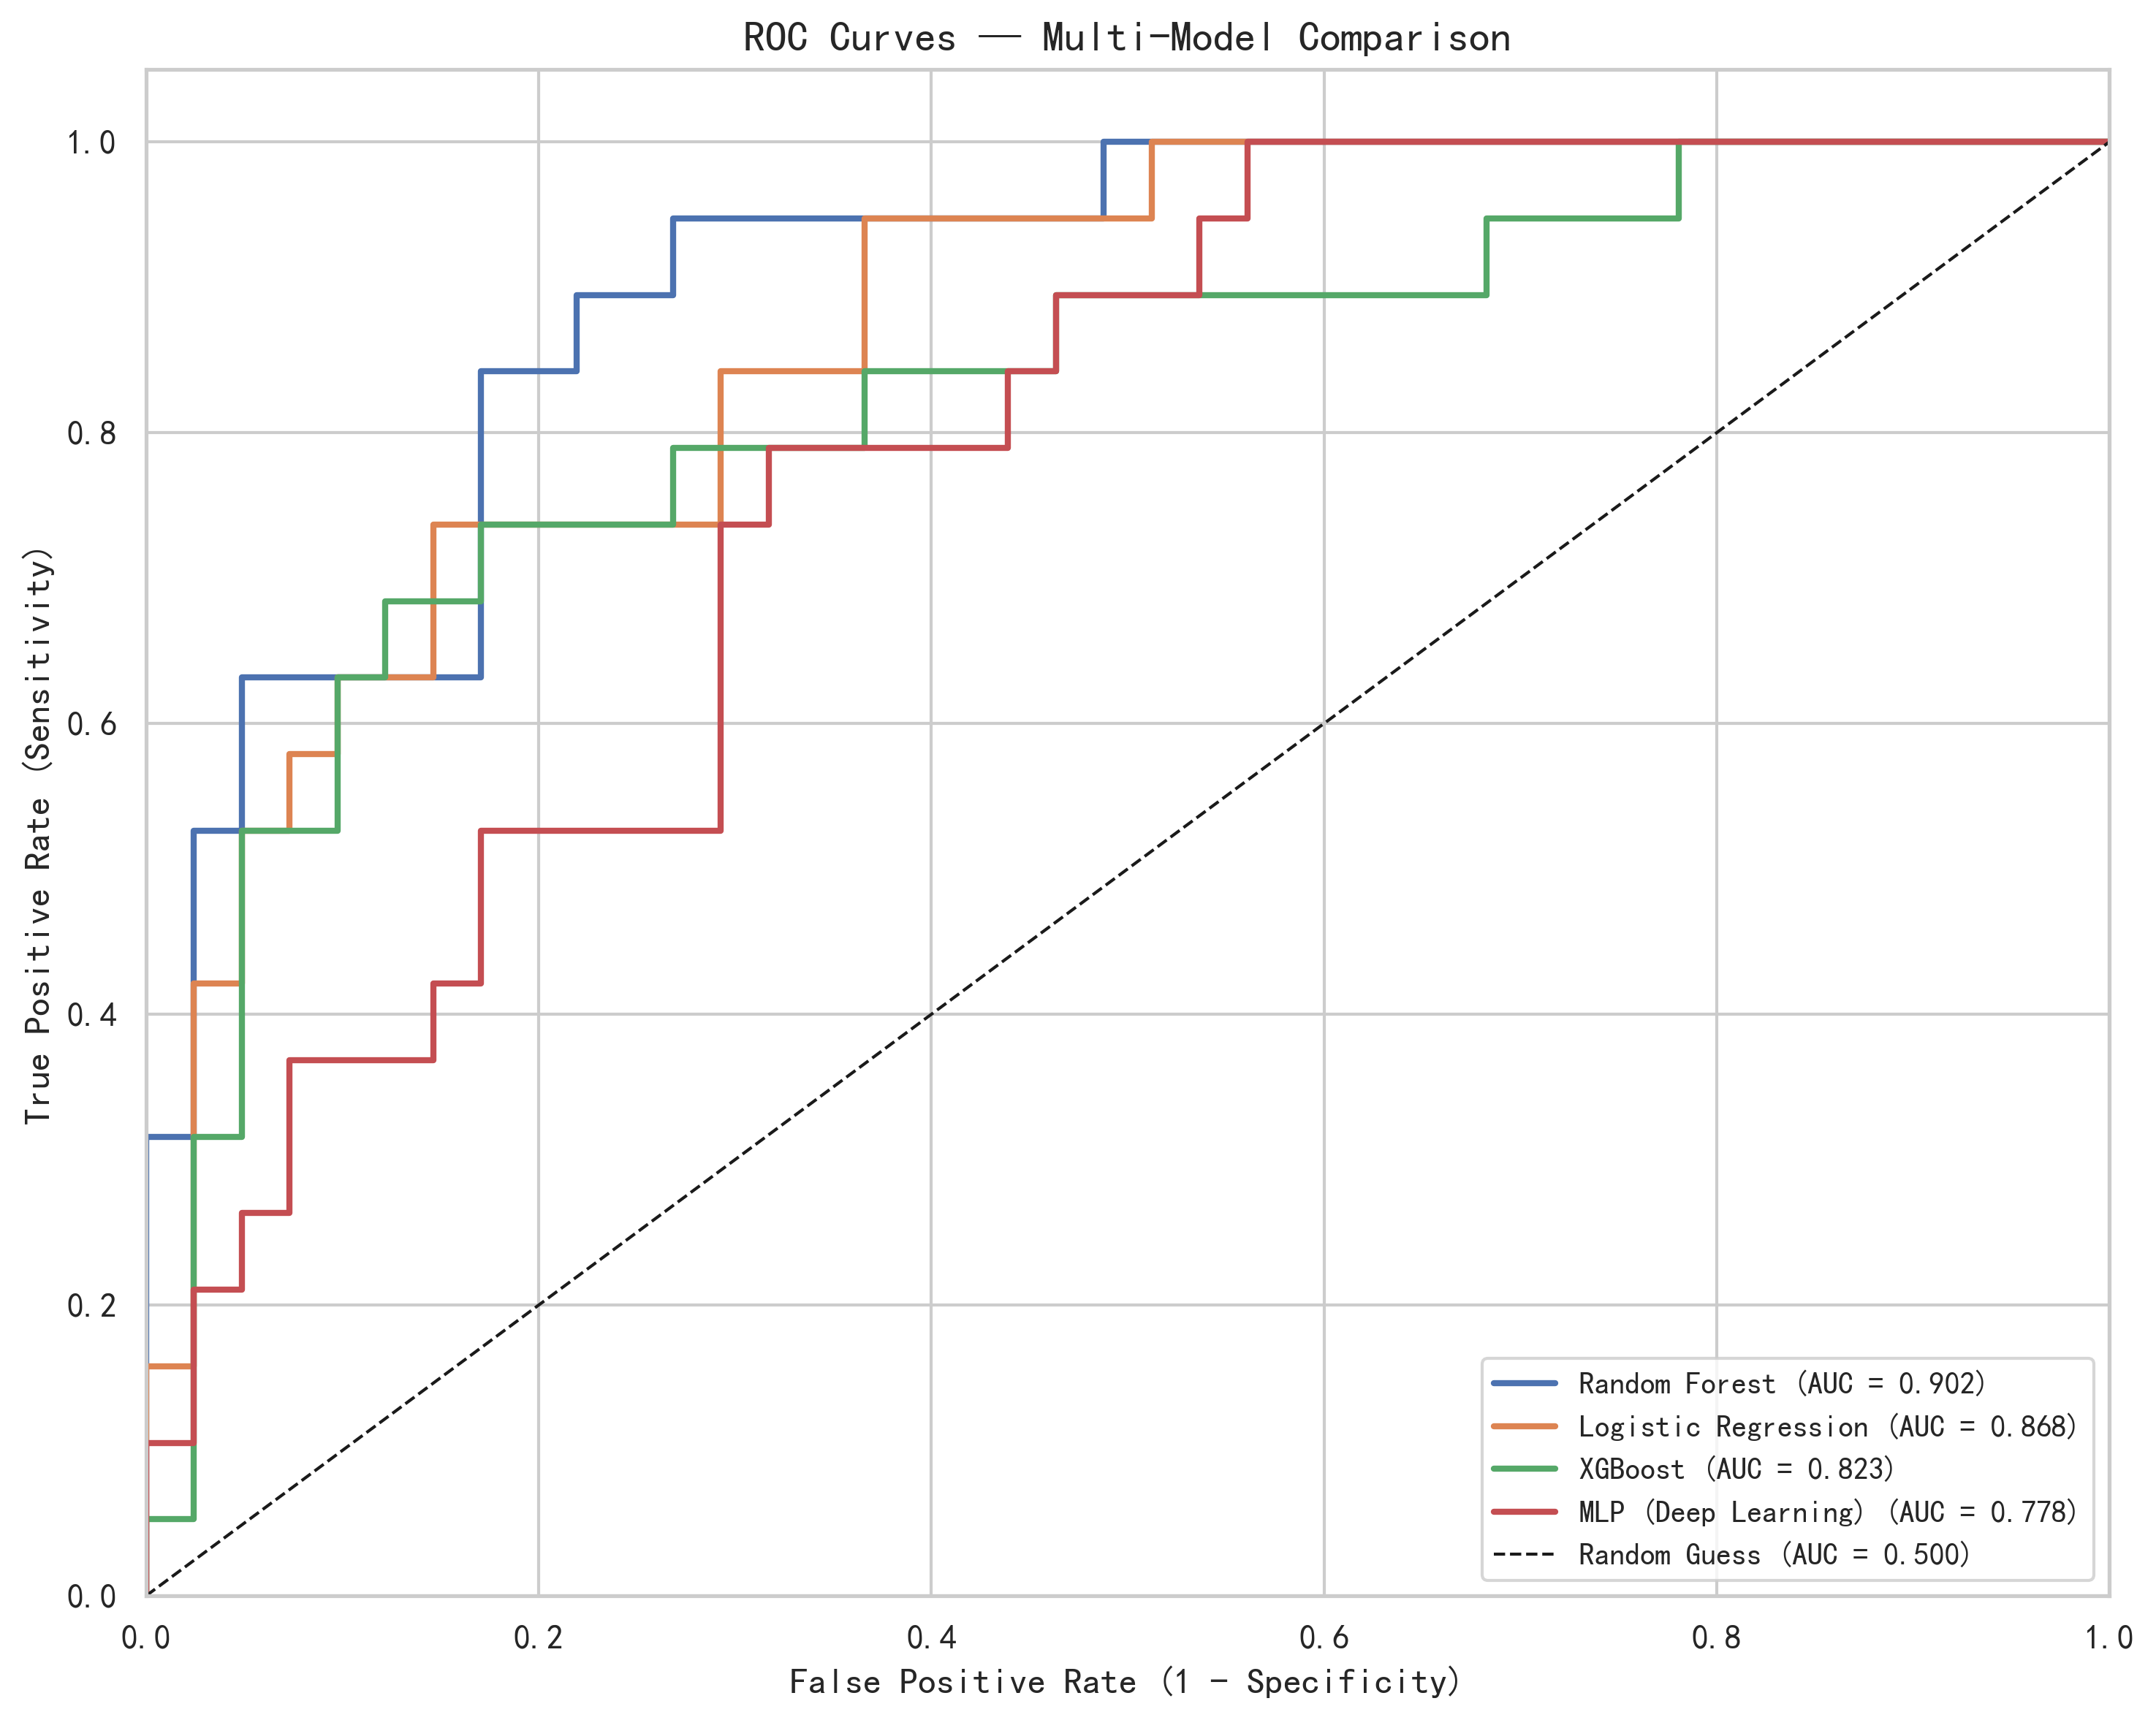
\includegraphics[width=0.85\textwidth]{roc_curves_comparison.png}
\caption{Receiver Operating Characteristic (ROC) curves for multi-model comparison. Random Forest achieved the highest AUC (0.9024), followed by Logistic Regression (0.8678), XGBoost (0.8678), and MLP (0.7279). The dashed diagonal line represents random classification performance (AUC = 0.500).}
\label{fig:roc_curves}
\end{figure}

The MLP deep learning model yielded the lowest AUC (0.7279) and a notably poor recall (0.2632), indicating that it missed a large proportion of actual death cases. This underperformance is consistent with known limitations of deep learning on small-sample tabular data ($N=299$): the network contains approximately 4000+ trainable parameters and is prone to converging to local optima or mild overfitting, whereas ensemble tree methods leverage bagging or boosting mechanisms for superior noise resistance and small-sample robustness.

\subsection{Cross-Validated Risk Factor Identification}

Three independent analytical methods consistently identified the same top risk factors for HF mortality:

\begin{enumerate}
    \item \textbf{Pearson correlation}: Time ($|r|=0.527$), SC ($|r|=0.388$), EF ($|r|=0.271$).
    \item \textbf{Welch's $t$-test}: Time ($p = 2.34\times10^{-22}$), SC ($p = 5.88\times10^{-10}$), EF ($p = 9.01\times10^{-6}$).
    \item \textbf{RF feature importance}: Time (0.362), SC (0.129), EF (0.122).
\end{enumerate}

This convergence across linear association, hypothesis testing, and nonlinear model-based importance provides robust evidence for the identified risk factors.

\subsection{Clinical Inference on New Patients}

To demonstrate the pipeline's clinical applicability, two virtual patients with contrasting risk profiles were evaluated.

\subsubsection{Case 1: High-Risk Cardiorenal Syndrome Patient}

Clinical profile: age 75, with anaemia, diabetes, hypertension, and smoking history; EF = 20\%, SC = 2.5\,mg/dL, SS = 130\,mEq/L, follow-up time = 4 days.

\begin{table}[H]
\centering
\caption{Predicted mortality probabilities for the high-risk patient (Case 1).}
\label{tab:case1}
\begin{tabular}{lc}
\toprule
\textbf{Model} & \textbf{Predicted Death Probability} \\
\midrule
Random Forest       & 92.00\% \\
Logistic Regression & 99.76\% \\
XGBoost             & 100.00\% \\
MLP (Deep Learning) & 86.11\% \\
\bottomrule
\end{tabular}
\end{table}

All four models reached high consensus ($>86\%$) on extreme mortality risk, consistent with severe left ventricular systolic dysfunction (EF = 20\%) and cardiorenal syndrome (SC = 2.5\,mg/dL).

\subsubsection{Case 2: Low-Risk Patient with Good Prognosis}

Clinical profile: age 45, no anaemia, no diabetes, no hypertension; EF = 55\%, SC = 0.8\,mg/dL, SS = 140\,mEq/L, follow-up time = 240 days.

\begin{table}[H]
\centering
\caption{Predicted mortality probabilities for the low-risk patient (Case 2).}
\label{tab:case2}
\begin{tabular}{lc}
\toprule
\textbf{Model} & \textbf{Predicted Death Probability} \\
\midrule
Random Forest       & 1.04\% \\
Logistic Regression & 0.13\% \\
XGBoost             & 0.00\% \\
MLP (Deep Learning) & 3.82\% \\
\bottomrule
\end{tabular}
\end{table}

All models converged on a very low mortality risk ($<4\%$), indicating well-compensated cardiac function and favorable prognosis.

%% ============================================================
\section{Discussion}
\label{sec:discussion}

\subsection{Model Performance and Methodological Implications}

The experimental results demonstrate that Random Forest achieves the best overall performance (AUC = 0.9024) on this small-sample structured clinical dataset, outperforming XGBoost (AUC = 0.8678), Logistic Regression (AUC = 0.8678), and MLP (AUC = 0.7279). This finding aligns with established evidence that ensemble tree methods are particularly well-suited for tabular data with limited sample sizes \citep{ali2023ml, uddin2019comparing}.

The suboptimal performance of the MLP is attributable to the high parameter-to-sample ratio inherent in deep architectures. Despite the incorporation of batch normalization, dropout regularization, and weight decay, the network's approximately 4000 parameters could not be reliably estimated from only 239 training samples. This observation provides a valuable methodological lesson: for small-sample tabular clinical data, traditional ensemble learning methods retain significant advantages in predictive accuracy and robustness.

\subsection{Clinical Interpretation of Risk Factors}

The three top risk factors identified through cross-validated analysis have clear clinical significance:

\textbf{Follow-up time (Time).} In survival-analysis data, a short follow-up duration associated with a death event typically indicates that the patient was already in a late or acute phase of the disease at admission, with rapidly escalating mortality risk. The strong negative correlation with the death event ($r = -0.53$) and the dramatic mean difference (70.89 vs.\ 158.34 days, $p < 0.001$) underscore the importance of early intervention for newly diagnosed HF patients.

\textbf{Serum creatinine (SC).} Creatinine is the gold-standard biomarker for renal function assessment. HF frequently triggers cardiorenal syndrome: when cardiac pump function deteriorates, systemic perfusion drops, glomerular filtration rate plummets, and serum creatinine rises sharply. Clinical literature indicates that HF patients with SC $> 1.5$\,mg/dL face significantly increased mortality. In our dataset, the deceased group had a significantly higher mean SC (1.48 vs.\ 1.12\,mg/dL, $p < 0.001$). This is consistent with previous findings that renal impairment is a strong independent predictor of all-cause mortality in HF \citep{chicco2020ml, ali2023ml}.

\textbf{Ejection fraction (EF).} EF quantifies the percentage of blood ejected from the ventricle per contraction and is the gold-standard indicator of left ventricular systolic function. Normal values range from 50\% to 70\%; values below 40\% define HF with reduced EF (HFrEF) \citep{austin2013}. A significantly reduced EF indicates that the heart can no longer maintain adequate peripheral tissue oxygenation, predisposing to malignant arrhythmias, cardiogenic shock, or multi-organ failure. The deceased group showed significantly lower EF (33.44\% vs.\ 40.20\%, $p < 0.001$).

It is worth noting that platelets and CPK, while showing moderate RF importance scores (ranked 5th and 7th), did not reach statistical significance in the $t$-test. This suggests their predictive contributions arise primarily through nonlinear interactions with other variables---a nuance that tree-based models capture effectively but univariate tests cannot.

\subsection{Comparison with Related Work}

Compared with Ali et al.\ \citep{ali2023ml}, who reported 97.78\% accuracy using RF with SMOTE oversampling and a 70/30 train-test split, our study employed a different preprocessing strategy (Winsorization instead of outlier removal, no SMOTE) and a 80/20 split ratio, resulting in a more conservative accuracy of 85.00\% but with a strong AUC of 0.9024. The risk factor rankings are broadly consistent: both studies identify SC and EF among the top features. Our study additionally incorporates a deep learning comparison and formal statistical testing to strengthen the evidence for feature relevance.

\subsection{Limitations and Future Work}

The primary limitation is the small dataset size ($N=299$). The class imbalance (32.1\% mortality) was addressed through stratified sampling but not through oversampling techniques. Future work should: (1)~validate the pipeline on larger, multi-center HF cohorts; (2)~explore advanced deep learning architectures designed for tabular data (e.g., TabNet, FT-Transformer); and (3)~incorporate time-series analysis for longitudinal clinical measurements.

%% ============================================================
\section{Conclusion}
\label{sec:conclusion}

This study established a multi-model prognostic assessment pipeline centered on Random Forest for HF mortality prediction. Experiments confirmed that on small-sample structured clinical data, the ensemble tree model (RF, AUC = 0.9024) outperforms gradient boosting (XGBoost, AUC = 0.8678), the linear model (LR, AUC = 0.8678), and deep learning (MLP, AUC = 0.7279).

Through Pearson correlation analysis, Welch's $t$-test, and RF feature importance---three independent cross-validation methods---the top three risk factors were identified as follow-up time, serum creatinine, and ejection fraction. These findings strongly corroborate established clinical knowledge regarding cardiorenal syndrome and left ventricular systolic dysfunction as major drivers of HF mortality.

The pipeline's clinical inference capability, demonstrated through individualized probability predictions for new patients, has potential scientific value for assisting clinicians in prognostic risk stratification of HF patients.

%% ============================================================
\section*{Declaration of Competing Interest}

The authors declare that they have no known competing financial interests or personal relationships that could have appeared to influence the work reported in this paper.

\section*{Data Availability}

The dataset is publicly available online as described by Ahmad et al.\ \citep{ahmad2017}.

%% ============================================================
\bibliographystyle{plainnat}

\begin{thebibliography}{99}

\bibitem[Chicco and Jurman(2020)]{chicco2020ml}
D.~Chicco and G.~Jurman.
\newblock Machine learning can predict survival of patients with heart failure from serum creatinine and ejection fraction alone.
\newblock \emph{BMC Medical Informatics and Decision Making}, 20(1):16, 2020.

\bibitem[Pocock et~al.(2006)]{pocock2006}
S.~J. Pocock, D.~Wang, M.~A. Pfeffer, S.~Yusuf, J.~J. McMurray, K.~B. Swedberg, J.~Ostergren, E.~L. Michelson, K.~S. Pieper, and C.~B. Granger.
\newblock Predictors of mortality and morbidity in patients with chronic heart failure.
\newblock \emph{European Heart Journal}, 27(1):65--75, 2006.

\bibitem[Ahmad et~al.(2017)]{ahmad2017}
T.~Ahmad, A.~Munir, S.~H. Bhatti, M.~Aftab, and M.~A. Raza.
\newblock Survival analysis of heart failure patients: A case study.
\newblock \emph{PLoS One}, 12(7):e0181001, 2017.

\bibitem[Ali et~al.(2023)]{ali2023ml}
M.~M. Ali, V.~S. Al-Doori, N.~Mirzah, A.~A. Hemu, I.~Mahmud, S.~Azam, K.~F. Al-tabatabaie, K.~Ahmed, F.~M. Bui, and M.~A. Moni.
\newblock A machine learning approach for risk factors analysis and survival prediction of Heart Failure patients.
\newblock \emph{Healthcare Analytics}, 3:100182, 2023.

\bibitem[Austin et~al.(2013)]{austin2013}
P.~C. Austin, J.~V. Tu, J.~E. Ho, D.~Levy, and D.~S. Lee.
\newblock Using methods from the data-mining and machine-learning literature for disease classification and prediction: a case study examining classification of heart failure subtypes.
\newblock \emph{Journal of Clinical Epidemiology}, 66(4):398--407, 2013.

\bibitem[Uddin et~al.(2019)]{uddin2019comparing}
S.~Uddin, A.~Khan, M.~E. Hossain, and M.~A. Moni.
\newblock Comparing different supervised machine learning algorithms for disease prediction.
\newblock \emph{BMC Medical Informatics and Decision Making}, 19(1):1--16, 2019.

\bibitem[Pocock et~al.(2013)]{pocock2013}
S.~J. Pocock, C.~A. Ariti, J.~J. McMurray, A.~Maggioni, L.~K{\o}ber, I.~B. Squire, K.~Swedberg, J.~Dobson, K.~K. Poppe, G.~A. Whalley, and R.~N. Doughty.
\newblock Predicting survival in heart failure: a risk score based on 39,372 patients from 30 studies.
\newblock \emph{European Heart Journal}, 34(19):1404--1413, 2013.

\bibitem[Zahid et~al.(2019)]{zahid2019}
F.~M. Zahid, S.~Ramzan, S.~Faisal, and I.~Hussain.
\newblock Gender based survival prediction models for heart failure patients: a case study in Pakistan.
\newblock \emph{PLoS One}, 14(2):e0210602, 2019.

\bibitem[Cho et~al.(2021)]{cho2021}
S.~Y. Cho, S.~H. Kim, S.~H. Kang, K.~J. Lee, D.~Choi, S.~Kang, S.~J. Park, T.~Kim, C.~H. Yoon, T.~J. Youn, and I.~H. Chae.
\newblock Pre-existing and machine learning-based models for cardiovascular risk prediction.
\newblock \emph{Scientific Reports}, 11(1):8886, 2021.

\bibitem[Ghosh et~al.(2021)]{ghosh2021}
P.~Ghosh, S.~Azam, M.~Jonkman, A.~Karim, F.~M. Shamrat, E.~Ignatious, S.~Shultana, A.~R. Beeravolu, and F.~De~Boer.
\newblock Efficient prediction of cardiovascular disease using machine learning algorithms with relief and lasso feature selection techniques.
\newblock \emph{IEEE Access}, 9:19304--19326, 2021.

\end{thebibliography}

\end{document}

\end{document}
